\section{\name: IO Root-of-Trust}
\label{sec:systemDesign}


In this section, we provide the technical details of \name integrity protection for IO devices.  

\subsection{System Components}
\label{sec:systemDesign:components}

Figure~\ref{fig:approachOverview} provides the highlevel approach overview of \name. The components of \name are the following:

\begin{mylist}
  \item \textbf{Host system.} The host system is completely compromised (hardware, OS and the installed applications) by the attacker.
  \item \textbf{\device.} The \device is connected to the input devices and sits between the host and the display. The \device is connected to the input devices over the \usb interface and connected to the host and the display over HDMI.
  \item \textbf{Input device.} The input devices such as the mouse, keyboard, touchpad, etc. are connected to the \device over \usb interface.
  \item \textbf{Display.} The display device is connected to the \device over HDMI interface.
  \item \textbf{Remote server.} The remote server is a trusted entity that serves the web application to the host system over \http. The remote server also creates a secure channel with the \device using the host as an untrusted transport. 
  
\end{mylist}

\subsection{Initialization} 
\label{sec:systemDesign:init}

There are two steps of initialization process: 

\begin{mylist}
  \item\textbf{IO initialization.} The \device initializes the mouse by instructing the host system to move the mouse pointer to the top right corner (moving to the first right and then up for an arbitrarily large value). As the \device has access to the frames that are displayed on the screen, it can verify if the mouse pointer is at the top-right corner of the screen or not. Then it instructs the host OS to bring it to the center of the screen.
  
  \item\textbf{Network initialization.} The \device connects to the remote server using \webusb or \webbt, effectively using the host as an untrusted transport. The \device and the server establishes a secure channel with the public certificates that are distributed before-hand.
\end{mylist}


\subsection{Communication Channel}
\label{sec:systemDesign:communicationChannel}

The communication channel between the \device and the remote server is constructed without employing any and separate hardware/software or web-browser extensions. \name two-way communication works out-of-the-box using JavaScript code and QR code decoding routine that runs on the \device. The \emph{downstream} channel, i.e., the data channel from the remote server and the \device relies in the HDMI channel. The remote server encodes the information in the webpage in QR code that is intercepted by the \device from the HDMI channel and decoded.

The \emph{upstream} channel, i.e., the data from the \device to the remote server is transmitted using the \name JavaScript snippet that is served by the remote web server. The \name JavaScript snippet uses a hidden text field to accept data coming from the \device. The \device emulates itself as a composite keyboard-mouse device when it is connected to the host. The \device emulates keystrokes that transmits encoded data to the \name JavaScript snippet that is sent to the remove server via \texttt{XMLHttpRequest} call.


\subsection{Key Establishment Protocol}
\label{sec:systemDesign:keyEstablishment}

\begin{figure}[t]
\centering
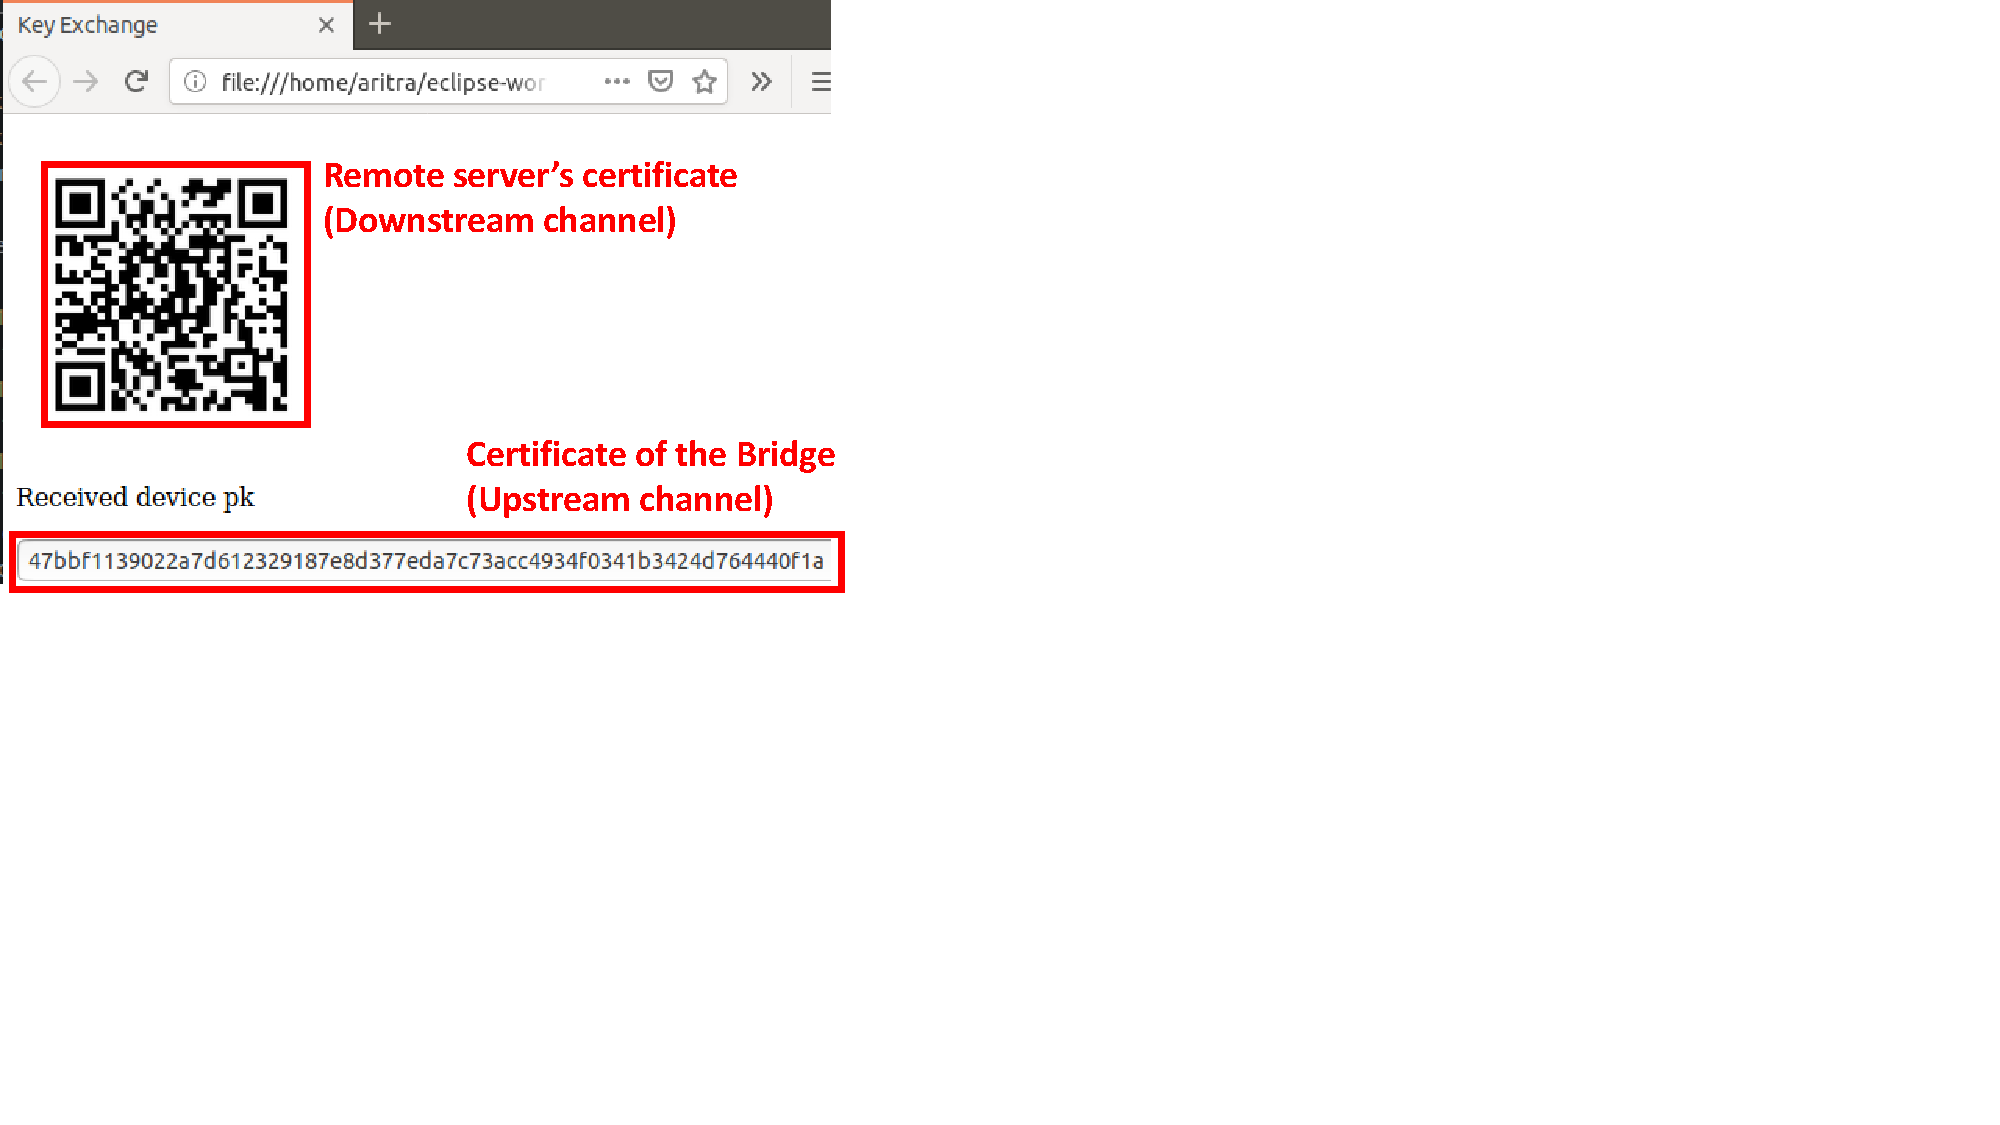
\includegraphics[trim={0 8cm 18cm 0}, clip, width=0.8\linewidth]{keyExchange.pdf}
\caption{\textbf{Key establishment.} A snapshot of the key exchange web page that is used to communicate the public certificates of the device and the remote server. This page only lasts for a few milliseconds, hence the page is practically invisible to the user.}
\label{fig:keyExchange}
\centering
\end{figure}

When the user opens up a webpage that supports \name mechanism, key exchange is the first step that is executed by the \device. Also the key exchange phase is crucial as the remote server also access if the user is in possession of a \device. An instance of the key exchange mechanism of \name is illustrated in Figure~\ref{fig:keyExchange}. The flow of the key exchange mechanism is as the following:

\begin{mylist}
  \item The remote web server serves the web page that shows a QR code that encodes the signed public key of the remote server. This page has a $5$ seconds time out.
  \item The device captures the frames and looks for a QR code. As soon as the device finds one, the device decodes the QR code and verifies it.
  \item If the verification is successful, the device emulates itself as a keyboard device to the host system. The device then encodes its public certificate to hexadecimal and send it as a keystroke to the host.
  \item The\name  JavaScript snippet looks for the keystrokes, and as soon as it gets a string of a specific length, it sends the key strokes to the remote server and the \name JavaScripts loads the webpage.
  \item In case the user is not in possession of a \device, the aforementioned step does not take place within the $5$ seconds timeout period. In that case \name JavaScript snippet concludes that the user does not have a \device. This allows the webpage to fallback to conventional web UIs that does not involves \device fro their operation.
\end{mylist}

After this, both the device and the remote server have each other's public certificates. Using these certificates, both the \device and remote server calculates the shared secret using Diffie-Hellman protocol~\footnote{Assume that $(g^x, x)$ and $(g^y, y)$ being the public-private key pair of the remote server and the \device respectively, where $g$ being a generator of a group $G$. The remote server sends a QR code that encodes a CA-signed $g^x$. The \device transmits signed $g^y$ to the remote server. Both the remote server and the \device computes $g^{xy}$ as the shared secret.}.



\begin{figure}[t]
\centering
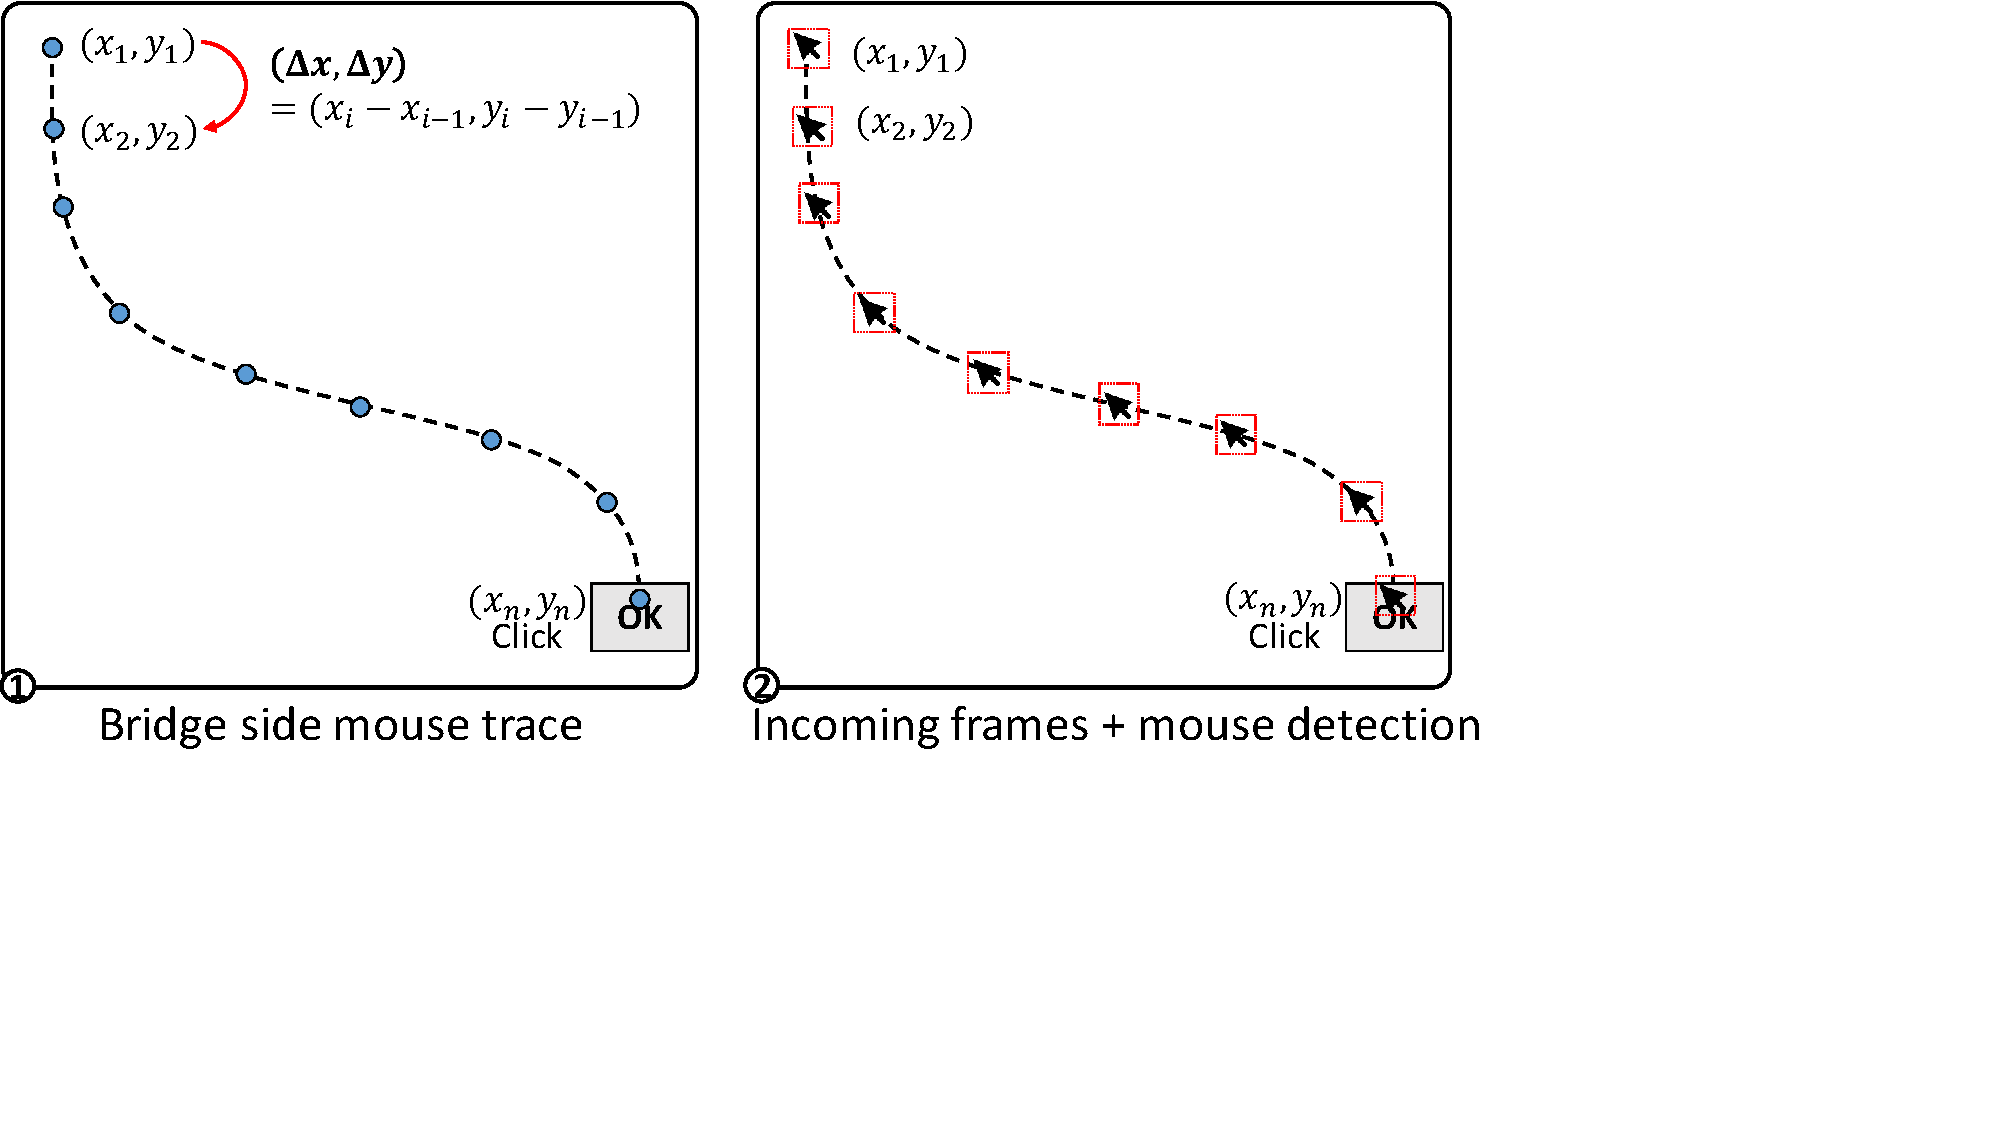
\includegraphics[trim={0 5.8cm 8cm 0}, clip, width=\linewidth]{mouseAnalysis.pdf}
\caption{\textbf{Proof-of-pointer.} The figure shows the high-level procedure of proof-of-pointer. The device knows the initial pointer position by sending a high mouse value to the host that puts the pointer on a specific corner $(x_0, y_0)$. \one The \device captures the raw mouse events ($\Delta x, \Delta y$) from the mouse that is attached to the \device. \two The \device captures the frames from the HDMI channel and checks into the designated pixel position $(x_i + \Delta x, y_i + \Delta y)$ if there exists a pointer.}
\label{fig:mouseAnalysis}
\centering
\end{figure}



\subsection{Analysis of HDMI Frames for Proof-of-pointer}
\label{sec:systemDesign:analysis}

The crucial property that \name provides is the user input integrity that combines both keyboard and mouse input. The integrity of the mouser input is nontrivial as one needs to know what the user sees on the screen. \name achieves this by intercepting the HDMI frames from the host system. The \device sits between the host and the display device (the monitor) and captures the frame to extract the cursor context. We call this property as the \emph{proof-of-pointer} where the \device generates the proof of the traces of the pointer. 

Figure~\ref{fig:mouseAnalysis} illustrates the high-level idea of the host system's HDMI frame analysis. To match the mouse polling rate with the display frame rate, the \device only queries the input device with the frequency of $60$ Hz. We assume that over the HDMI channel the host system sends frames at the rate of $60$ fps. We define the mouse trace as the time series $(\Delta x_i = |x_{t_{i-1}} - x_{t_{i}}|, \Delta y_i=|y_{t_{i-1}} - y_{t_{i}}|)$ delta co-ordinates: $\{(\Delta x_1, \Delta y_1), (\Delta x_2, \Delta y_2), \ldots, (\Delta x_n, \Delta y_n)\}$ from time $\{t_1, t_2, \ldots, t_n\}$. $x_{t_{i}}$ and $y_{t_{i}}$ denote the pixel position of the mouse pointer on the screen at time $t_i$. At the time of initialization, the \device pushes the mouse at the left-upper corner of the screen. hence $(x_0, y_0) = (0, 0)$.  
Note that a mouse only provides displacement over $x$ and $y$ coordinates. This corresponds that at time $t_i$ the mouse reported $(\Delta x_i, \Delta y_i)$ displacement to the \device. Assume that the frames coming from the host system to the \device are: $\{f_1, f_2, \ldots, f_n\}$ over the same time interval $(t_1, t_2,\ldots t_n)$. At time $t_i$, the \device looks into the frame $f_i$ and draws a square centered at $(x_i, y_i)$ with sides of length $X$ (enough to cover a mouse cursor~\footnote{in our evaluation we saw that a 30 px $\times$ 30 px can cover the default mouse pointer provided by Ubuntu.}). Then the \device checks if there exists a mouse inside this square or not. In case there exists a mouse cursor, the \device allows further user interactions otherwise it stops all the communications and shows an error on display.


\begin{figure*}[t]
\centering
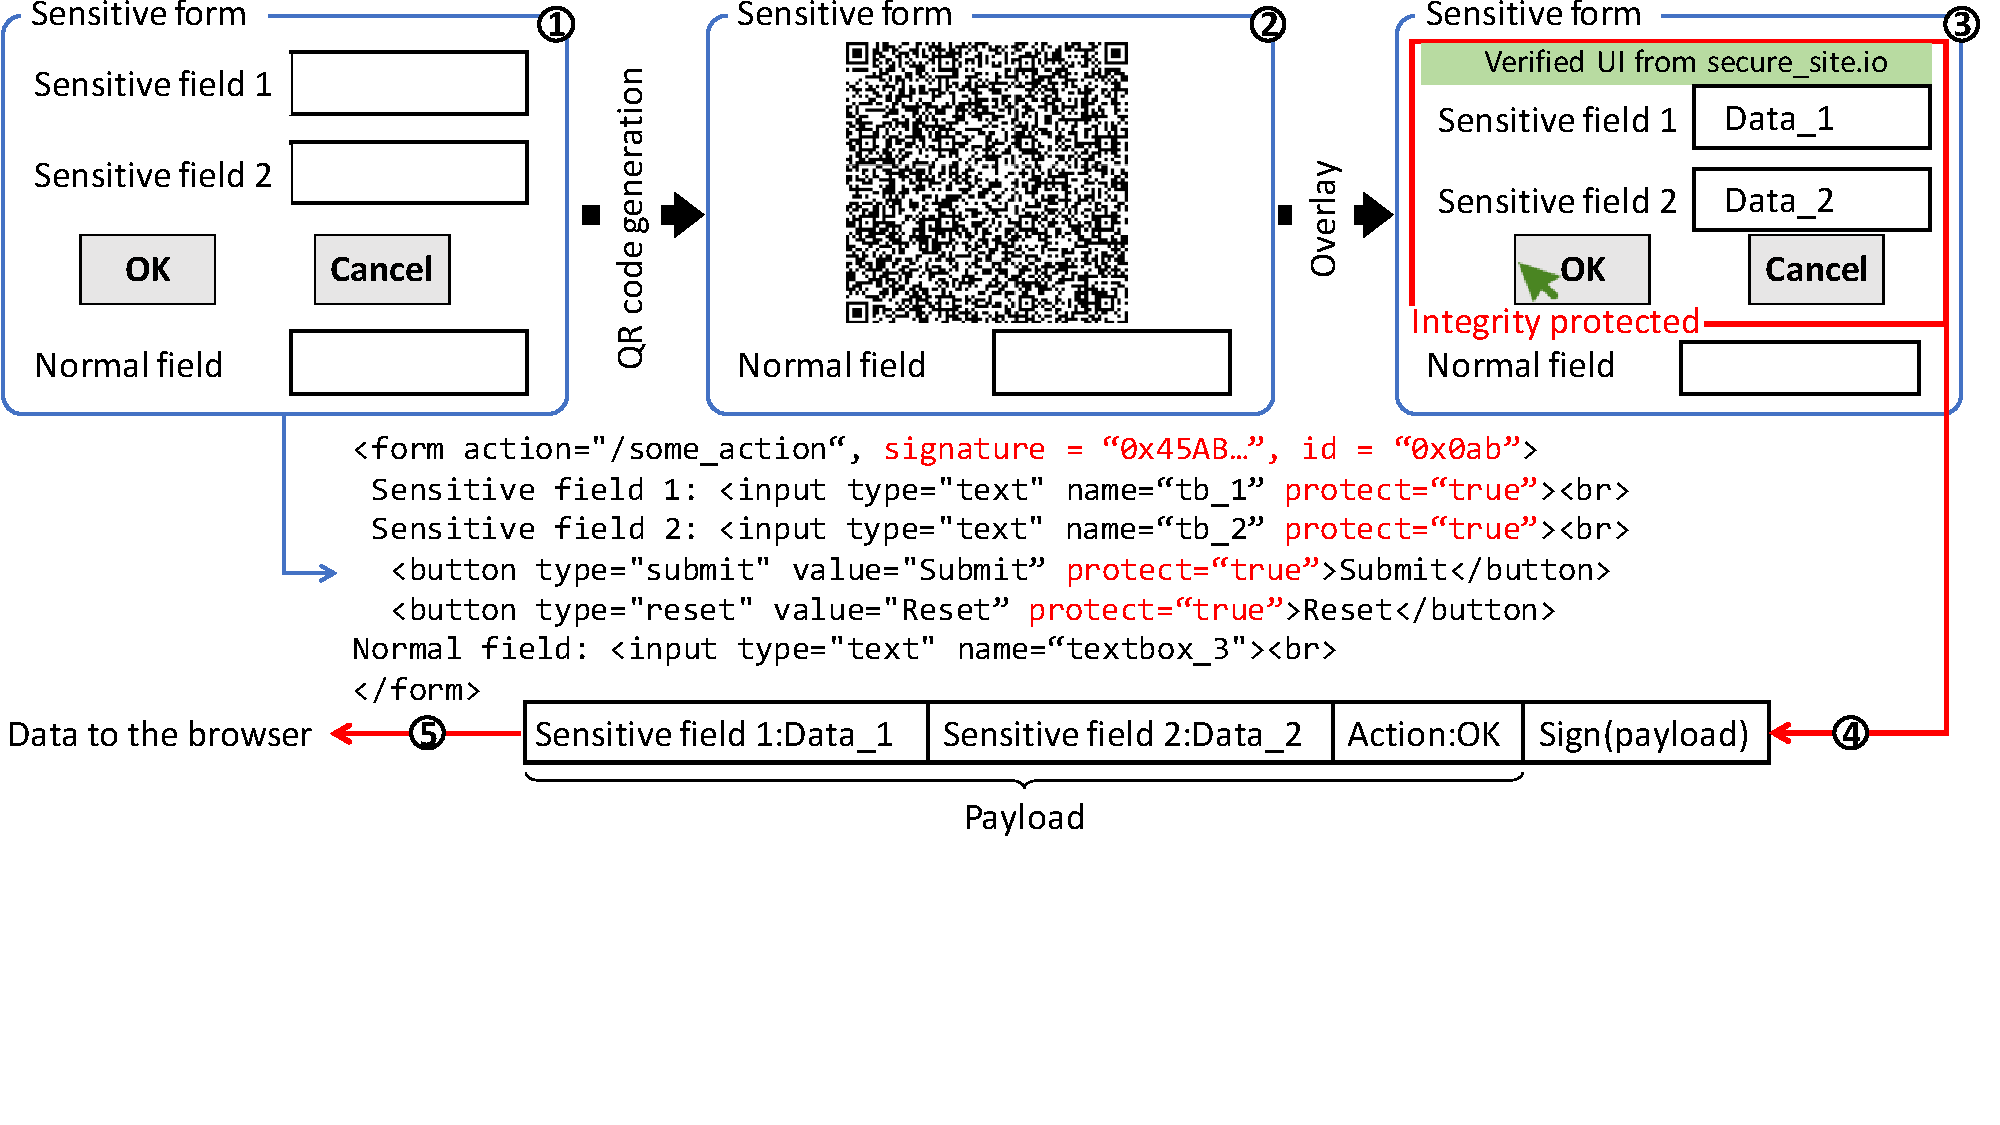
\includegraphics[trim={0 4cm 0 0}, clip, width=0.85\linewidth]{formTransform.pdf}
\caption{\textbf{Transformation of UI elements.} Automated transformation of the UI elements (\one) by the \name JavaScript snippets that detects the presence of the device. The corresponding \html source shows the UI elements that requires integrity/privacy protection. These UI elements are transformed to a QR code (\two). The QR code encodes a UI specification that recreates the transformed UI. Specification~\ref{snippet:UISpecification} shows corresponding UI specification that is created by the \name \js code. The QR code is then decoded and overlaid (\three) on the HDMI stream by the \device. Upon user's action on the overlaid UI elements, the device signs all the input data and send them to the remote server. As the rendered UI is generated and overlaid by the \device, it also ensures the integrity of the Ui elements. Note that the intermediate QR code transformation (\two) is not visible by the user as it is decoded instantaneously by the device.}
\label{fig:transformation}
\end{figure*}


\subsection{Transformation of UI Elements for Proof-of-Action and Proof-of-UI}
\label{sec:systemDesign:transformation}


In this section, we describe the most crucial part of the \name solution: transformation of the user interface (UI) elements. This transformation provides two security property i) proof-of-action that ensures integrity of the user input, and ii) proof-of-UI that ensures secure display. Before describing the transformation, we first provide a strawman solution that is based in text/image analysis that we opted not no use due to several drawbacks.   

\begin{figure}[!htpb]
\centering
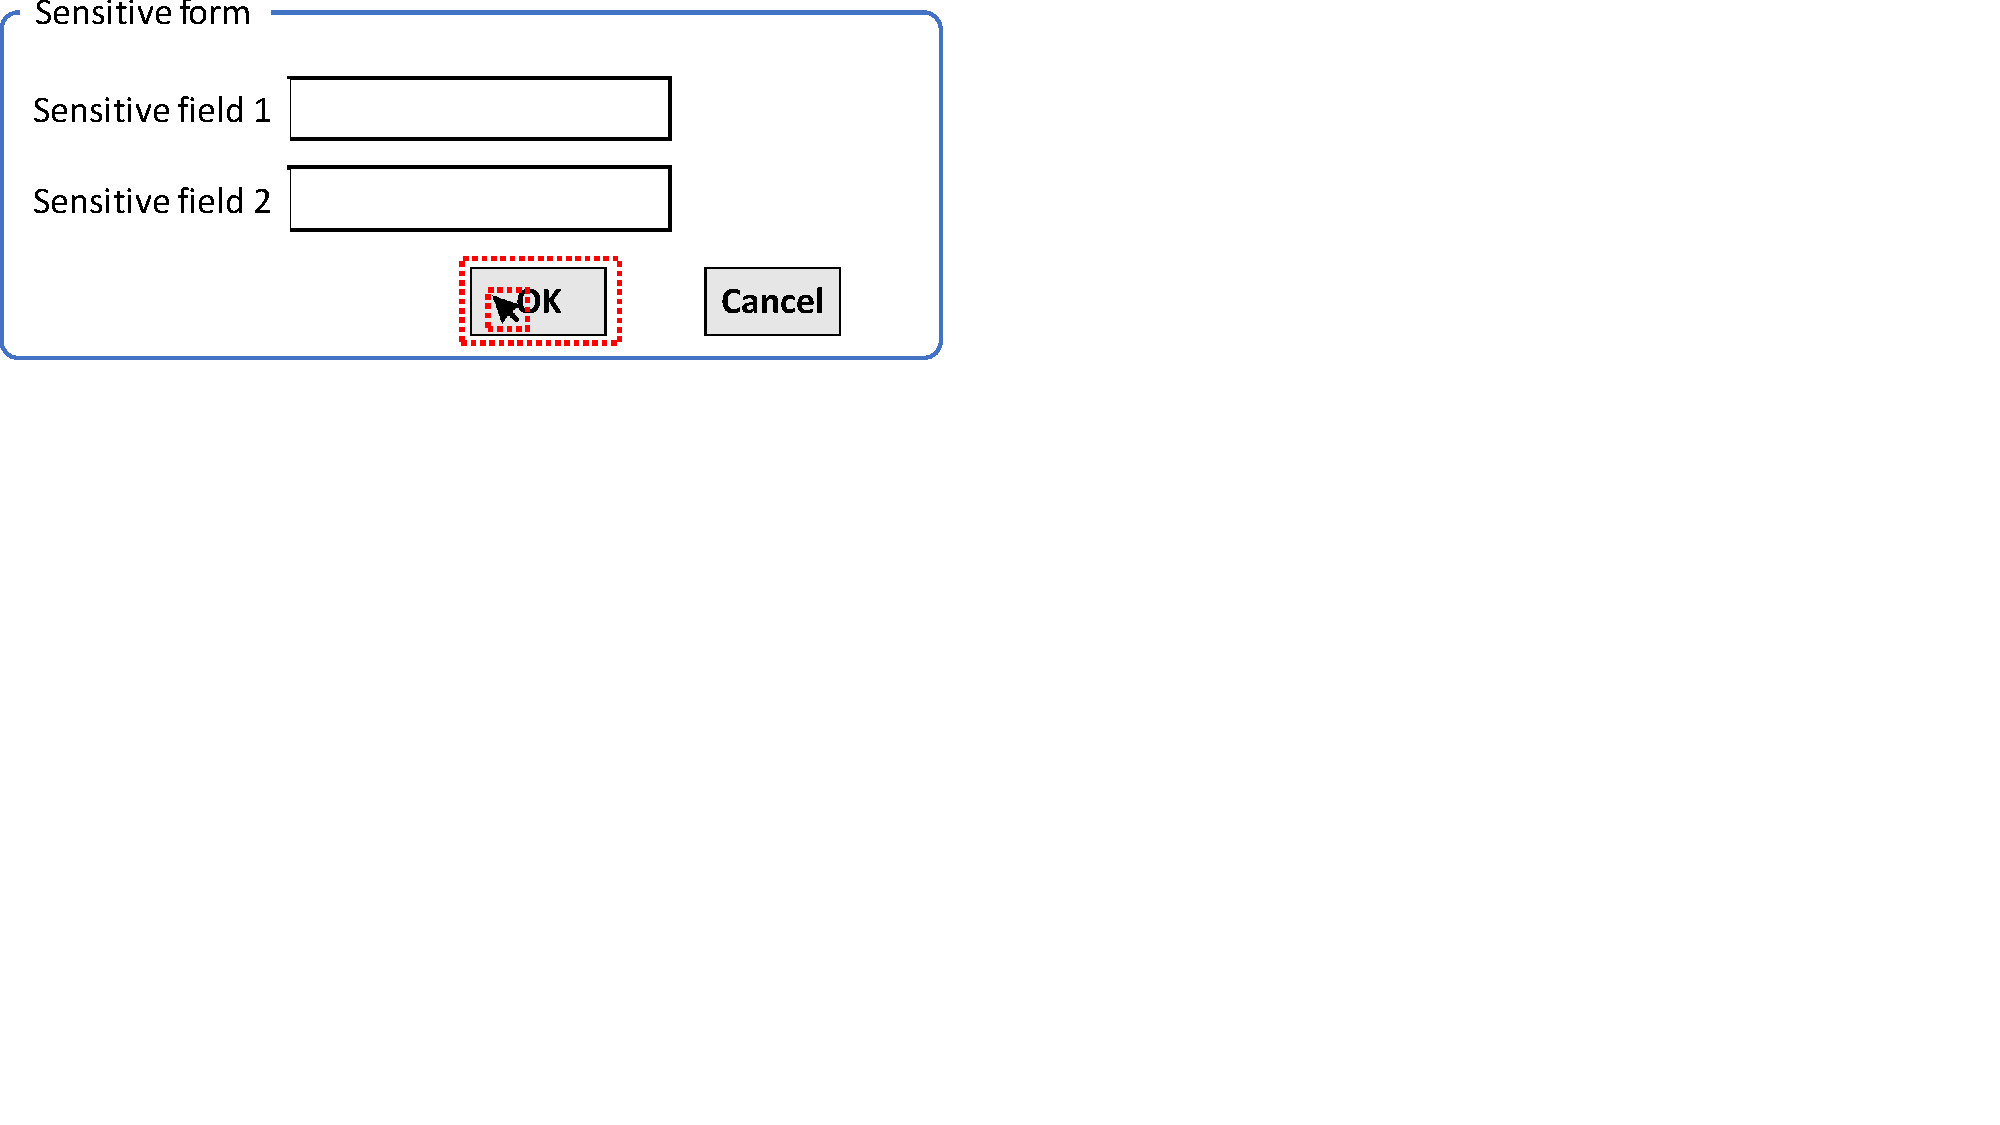
\includegraphics[trim={0 12.5cm 21cm 0}, clip, width=0.65\linewidth]{uiDetect.pdf}
\caption{\textbf{Potential solution to understand the context of an UI element}. The earlier version of the \name solution employs image analysis to detect the UI element leveraging edge detection and optical character recognition (to extract the labels on the UI element). The solution suffers from lack of robustness where the \device sometime fails to correctly classify the UI elements/labels due to mouse position or colors.}
\label{fig:uiDetect}
\centering
\end{figure}

\subsubsection{Potential solution and its drawback} One of the potential solution that we thought of is to use image and text analysis to understand the semantics of the Ui elements. In Figure~\ref{fig:uiDetect} we illustrate on example scenario where the \device extract the context of the mouse position when a user clicks. This involves the \device to take a truncated screen-shot from the HDMI frame and use image analysis to classify that the user clicks on a button. The \device also uses character recognition technique to extract the label of the button. Further investigation and prototype implementation shows two primary drawbacks of this solution:


\begin{mylist}
  \item \textbf{Robustness.} Previous research works such as~\cite{lukaSpoof,Chen:2010:DVS:1754393.1754394} propose detection of phishing attack by visually analyzing the web interface of the mobile applications. All of these proposed methods fail to achieve 100\% accuracy in the real world scenarios. Our prototype implementation alo confirm that the method lacks robustness in the real life as most of the time the \device fails to either recognize the UI elements or extract the label from the UI elements properly despoite of using state-of-the-art image/text analysis tools~\cite{opencv}.
  \item \textbf{Performance.} The image/text analysis is CPU intensive and causes low number of frame output by the \device. Commonly used image analysis frameworks such as OpenCV~\cite{opencv} is CPU intensive and it hard to achieve $24$ fps after operation on the \device that is implemented on a ARM-based Raspberry Pi.
\end{mylist}


\subsubsection{UI transformation based approach} After the establishment of the secure channel between the device and the remote server, the \name JS snippet that is served with the webpage transform the UI elements that requires protection. We illustrate the method of UI transformation in Figure~\ref{fig:transformation}. The entire process has two phases: \emph{transformation}, and \emph{overlay}.


\lstset{language=JSON, frame=tb, caption=\textbf{Protected UI specification language.} The UI specification shows the JSON formatted UI specification that is encoded into a QR code. The specification is generated from the \html source that are tagged as protected from the developers. The example specification is generated from the \html source that is provided in corresponding UI in Figure~\ref{fig:transformation}., label=snippet:UISpecification, firstnumber =1}
\begin{figure}[t]
\begin{lstlisting}[mathescape=true]
{ "formId": "form1",
  "formName": "form1",
  "ui": [{ "id":"textbox_1",
     "type":"textbox",
     "label":"Sensitive field 1",
     "text":"secret data 1"},
   { "id":"textbox_2",
     "type":"textbox",
     "label":"Sensitive field 2",
     "text":"secret data 2"},
   {"id":"OK_button",
     "type":"button",
     "trigger":"true",
     "label":"OK"},    
   {"id":"Cancel_button",
     "type":"button",
     "trigger":"false",
     "label":"Cancel"}]}
\end{lstlisting}
\end{figure}

\begin{mylist}
\item \textbf{Transformation.} The transformation of the web page UI elements are handled by the \name JavaScript\footnote{In the prototype implementation on \name, we use QRCode.js, a \js library to produce QR codes} snippet that is served from the remote server. UI elements that require integrity protection can be marked by the developers in the \html source. As illustrated in Figure~\ref{fig:transformation}, the \html UI elements that have additional attribute \texttt{protect=``true''} requires integrity protection from the \device. The transformation phase is between \one and \two in Figure~\ref{fig:transformation} where the \name JavaScript snippet transforms the UI elements to a UI specification language in a QR code that can be interpreted by the \device. The UI specification corresponding to the \html source (in Figure~\ref{fig:transformation}) is provided in Specification~\ref{snippet:UISpecification}.

\item \textbf{Overlay.} Overlay is the next phase where the QR code that embeds the UI specification is interpreted by the \device and overlaid on the HDMI stream. The overlay faithfully recreates the UI to prevent any alteration in the user experience. The \device overlay is depicted in \three in Figure~\ref{fig:transformation}. The \device come with a small interpreter routine that converts the UI specifications to bitmaps that are then overlaid on the HDMI stream. The specification also contains the location and the size details (omitted from the Specification~\ref{snippet:UISpecification}). The \device uses this information to determine the specific UI element over which the user has her mouse pointer. As the \device parses all the HDMi frames for QR code, the overlay does not get interrupted by scrolling.
\end{mylist}

\subsubsection{Proof-of-UI} \emph{proof-of-UI} is the output integrity property that ensures the integrity of the UI elements and the data corresponding to them that are sent by the remote server. As the specification sent by the server is signed, the \device generates the integrity and authenticity of the UI elements on the web page. Note that the \device always draws on top of the frames that are rendered by the compromised host. This way, the overlaid UI is always visible by the user on display. As the UI is generated as per the specification sent from the remote server, the \device ensures UI integrity.

\subsubsection{Proof-of-action} After the UI elements are correctly overlaid on the screen, the users can interact with the elements as if there is no alternation. The \device understands the semantics of all the generated UI elements, such as when a user selects a text box and types on her keyboard, the \device intercepts all the keyboard strokes and overlays the characters on the UI. When the user clicks on the \texttt{OK} button on the overlay, the device gathers all the intercepted keyboard and mouse events, signs them and send them to the remote server. One example of the proof-of-action is depicted in Figure~\ref{fig:transformation} that shows the payload that the \device sends to the server. Along with the keyboard data that is provide by the user, the \device also attaches the proof that the user indeed clicked on the \texttt{OK} button that leads to the action. Detailed description how the input is recorded and committed is presented in Section~\ref{sec:systemDesign:commit}.

\begin{figure}[t]
\centering
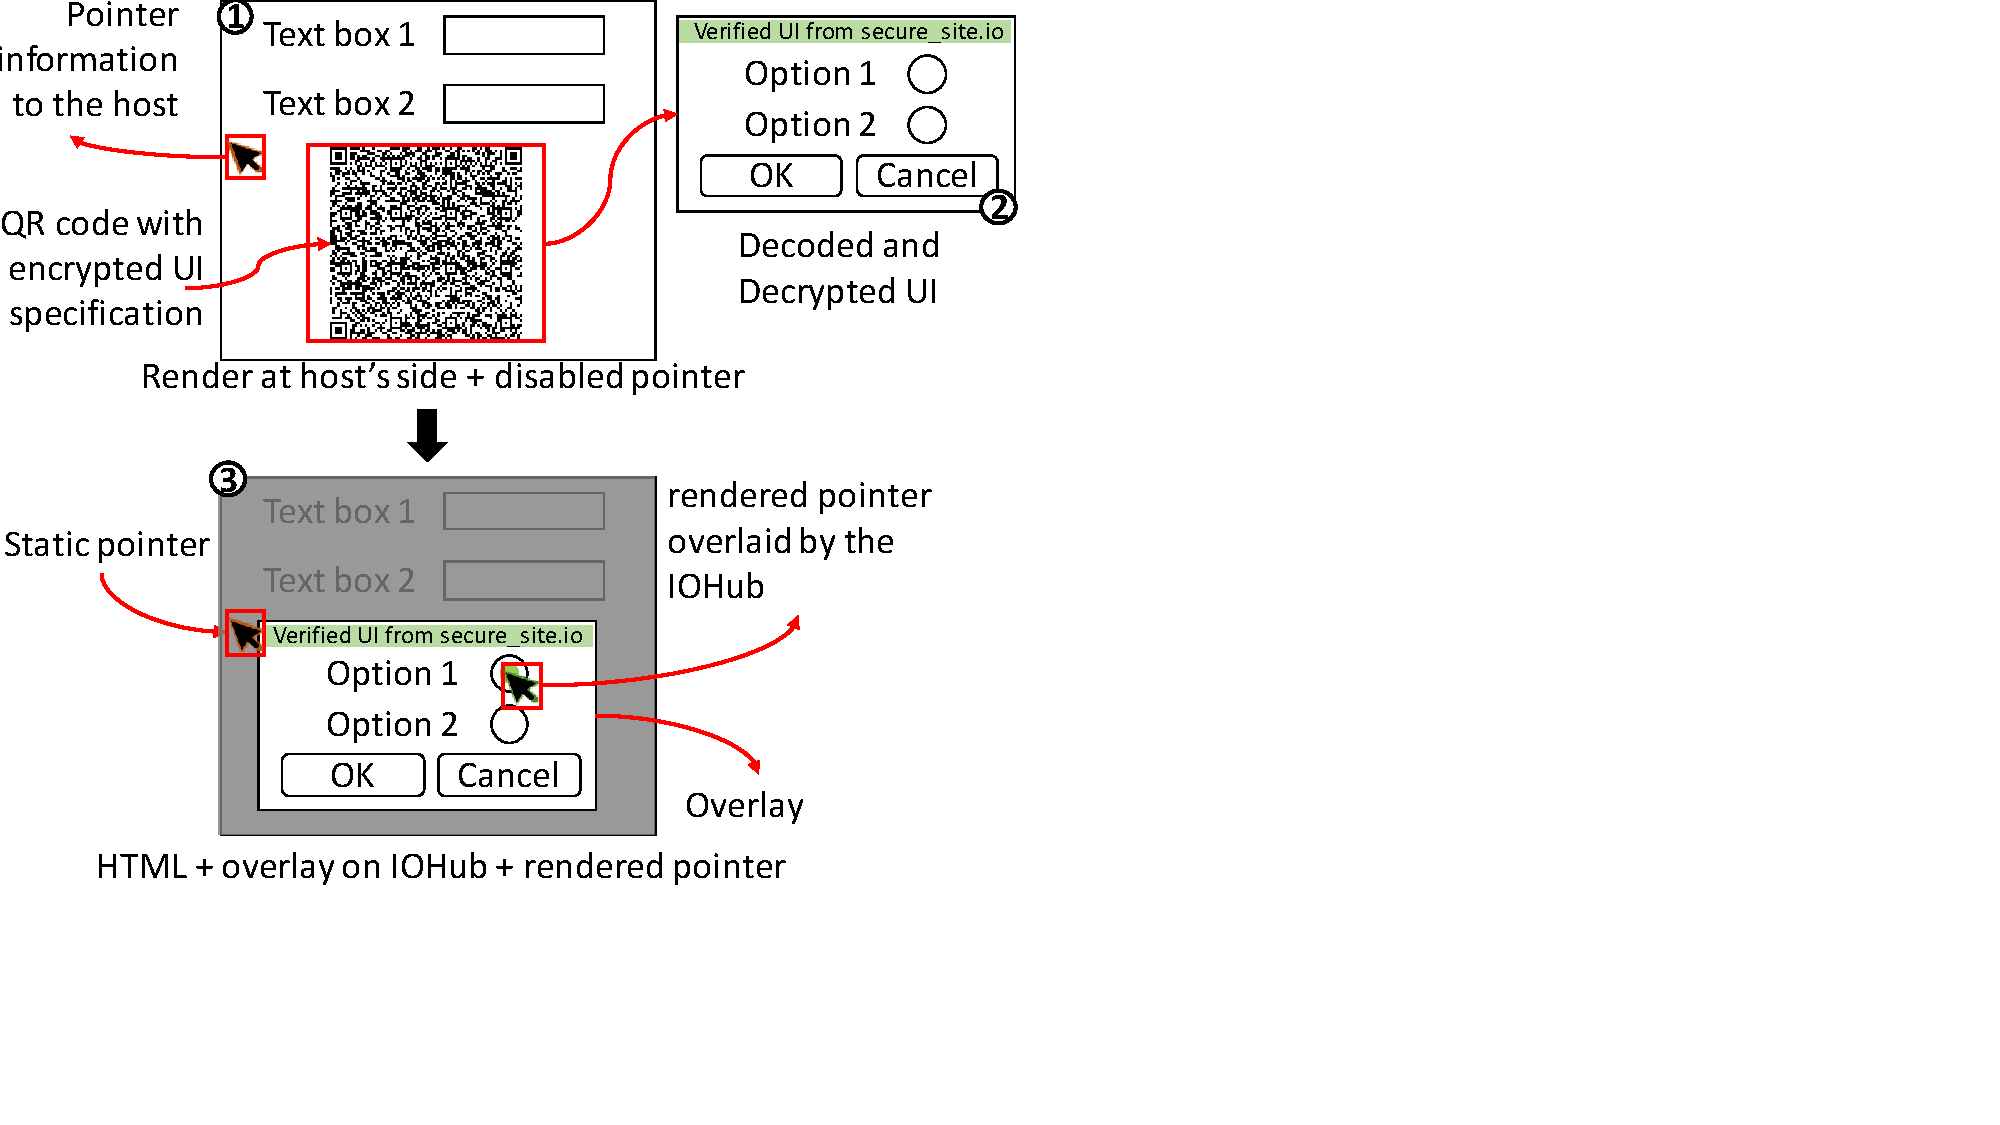
\includegraphics[trim={0 3cm 16.5cm 0}, clip, width=0.85\linewidth]{activityPrivacyRender.pdf}
\caption{\textbf{Privacy of the UI and the pointer.} The figure shows how \name achieves the privacy of the UI elements and the mouse pointer in the presence of a compromise host. The upper screenshot shows the host's view of the display while the lower one shows the user's view. The host can only see a QR code where the specification is encrypted by the \tls session key between the \device and the remote server. The user sees the decoded and overlaid UI objects that are retrieved from the QR code sent by the remote server (as described in Section~\ref{sec:systemDesign:transformation}).}
\label{fig:activityPrivacy}
\centering
\end{figure}



\lstset{language=HTML, frame=tb, caption=\textbf{HTML page from the remote server that contains the encrypted UI specification for IO privacy.} , label = snippet:encryptedHTML, firstnumber =1}
\begin{figure}[t]
\small
\begin{lstlisting}[mathescape=true]
<form action="/some_action">
  First name:<br>
  <input type="text" name="First name">
  <br> Last name:<br>
  <input type="text" name="name">
  <encrypted>
  [encrypted QR code specification]
  </encrypted>
  <input type="submit" value="Submit">
  <script>
  [javaScript that outputs encrypted QR code]
  </script>
</form> 
\end{lstlisting} 
\end{figure}


\subsection{Input \& Output Privacy}
\label{sec:systemDesign:mousePrivacy}


In the previous section (Section~\ref{sec:systemDesign:transformation}) we describe how the \name \js and the \device together transform and overlay the UI to ensure the integrity of the UI and the input data. Similar mechanism can be used to fully hide the input and output from an attacker-controlled host. For input we consider two cases i) the raw input to the remote server that is provided by the user from her input device, and ii) the mouse movement which is not the direct input to the remote server but ultimately leads to sending input to the remote server. To facilitate this, the remote server sends a encrypted UI spec as shown in the HTML snippet~\ref{snippet:encryptedHTML}. The key of the encryption is the session \tls key between the remote server and the \device (detailed key exchange process is described in Section~\ref{sec:systemDesign:keyEstablishment}). The \device stops forwarding any input made by the user as soon as the user enters the overlaid area. To keep the user experience consistent, the \device also overlays  

The \name \js convert this specification to a QR code that is intercepted, decoded and decrypted by the \device. The overall flow of the system is shown in Figure~\ref{fig:activityPrivacy}.  


\subsection{Secure Attention Sequence}
\label{sec:systemDesign:SAS}

Secure Attention Sequence (SAS) is a sequence of actions\footnote{Such as keystrokes \texttt{Ctrl+Alt+Del} that allows the user to provide her credential} executed by the user that is completely trustworthy. SAS prevents an untrusted system to trigger an event that is otherwise sensitive to the user. Note that SAS is a well-researched topic in the context of UI/UX design. \name uses off-the-shelf SAS mechanism and adapts it into the system. 

\name provides a mechanism for SAS where the user forces the \device to highlight the overlaid UI and the mouse pointer location. SAS eliminates any possibility that the attacker either i) create fake UI elsewhere in the screen that may trick the user into submitting sensitive information, or ii) spawn a fake mouse pointer to trick the user into clicking into a different location. To protect against such scenarios, \device also provides SAS using which the user can highlight the overlaid UIs and the mouse pointer on display. As the \device overlays on the HDMI frames, the attacker can not manipulate any overwriting by rendering anything on top of them. 
There are to SAS mechanisms that \name employs. One is intrinsic to the user action. When the user moves her mouse, the \device briefly outlines the overlay UI. The other SAS mechanism is when the user presses a button on the \device, the \device dims the rest of the part of the display except the legitimate mouse pointer and the overlaid UIs. By doing so, the user can easily discriminate the secure UIs and the legitimate mouse pointer.
 

\subsection{Committing User Input}
\label{sec:systemDesign:commit}

When the user finishes providing her input over the input device (mouse and keyboard), the \device commits these values to the remote server. The commitment is executed by providing the signed input values to the remote server. The commitment procedure is illustrated in Figure~\ref{fig:transformation}. The commitment has two phases: \emph{record} and \emph{commit}.

\myparagraph{Record} When user provides any information on the rendered overlay UI elements (such as textbox, button, slider, radio button, etc.), the \device records that in a (key, value) pair where the key is the identifier of the UI element (\texttt{id} in Specification~\ref{snippet:UISpecification}) and the value is the user provided value. The \texttt{type} of the UI elements determine what information to record. For example, the \device records all the keystrokes when a textbox is selected, the value corresponding to the position of the slider is recorded when the user interacts with a slider, etc. One example of the recording of the input data corresponding to the UI illustrated in Figure~\ref{fig:transformation} and Specification~\ref{snippet:UISpecification} is: 
\begin{align*}
Record = & (textbox\_1, Data\_1);(textbox\_2,Data\_2)
\end{align*}

\myparagraph{Commit} In the commitment phase, the \device waits for the user to operate on a UI element which has a \texttt{trigger} capability. For example, in Specification~\ref{snippet:UISpecification}, the \texttt{OK} and the \texttt{cancel} buttons have an attribute \texttt{trigger}. This attribute can take either \texttt{true} (corresponding to \texttt{OK}) or \texttt{false} (corresponding to \texttt{Cancel}) value that denotes that the the button can submit the values that are provided by the user or abort the form altogether. When the user performs some actions on the \texttt{trigger} enabled UI elements, the \device sends the signed recorded value to the \name JavaScript snippet. The \name \js snippet then sends these information to the remote server by a \texttt{XMLHttpRequest} call. The commit phase also makes sure that the user actually moves her mouse pointer from else where on the screen to the UI element using the proof-of-pointer mechanism described in Section~\ref{sec:systemDesign:analysis}. Apart from clicking, the user may hit \texttt{enter} that also trigger the \device to submit the form. 


\subsection{Server-side Computation}
\label{sec:systemDesign:serverSide}

After the \device commits the input records to the remote server, the remote server verifies the input with the data that is submitted by the browser running on the compromised host. The browser sends a \http packet to the server that contains the form data submitted by the user. On the other hand, the \device sends the signed input traces from the user via the \tls channel between the \device and the remote server. The server verifies the signature and accepts the input if they are identical to the data submitted by the browser.

\begin{figure}[t]
\centering
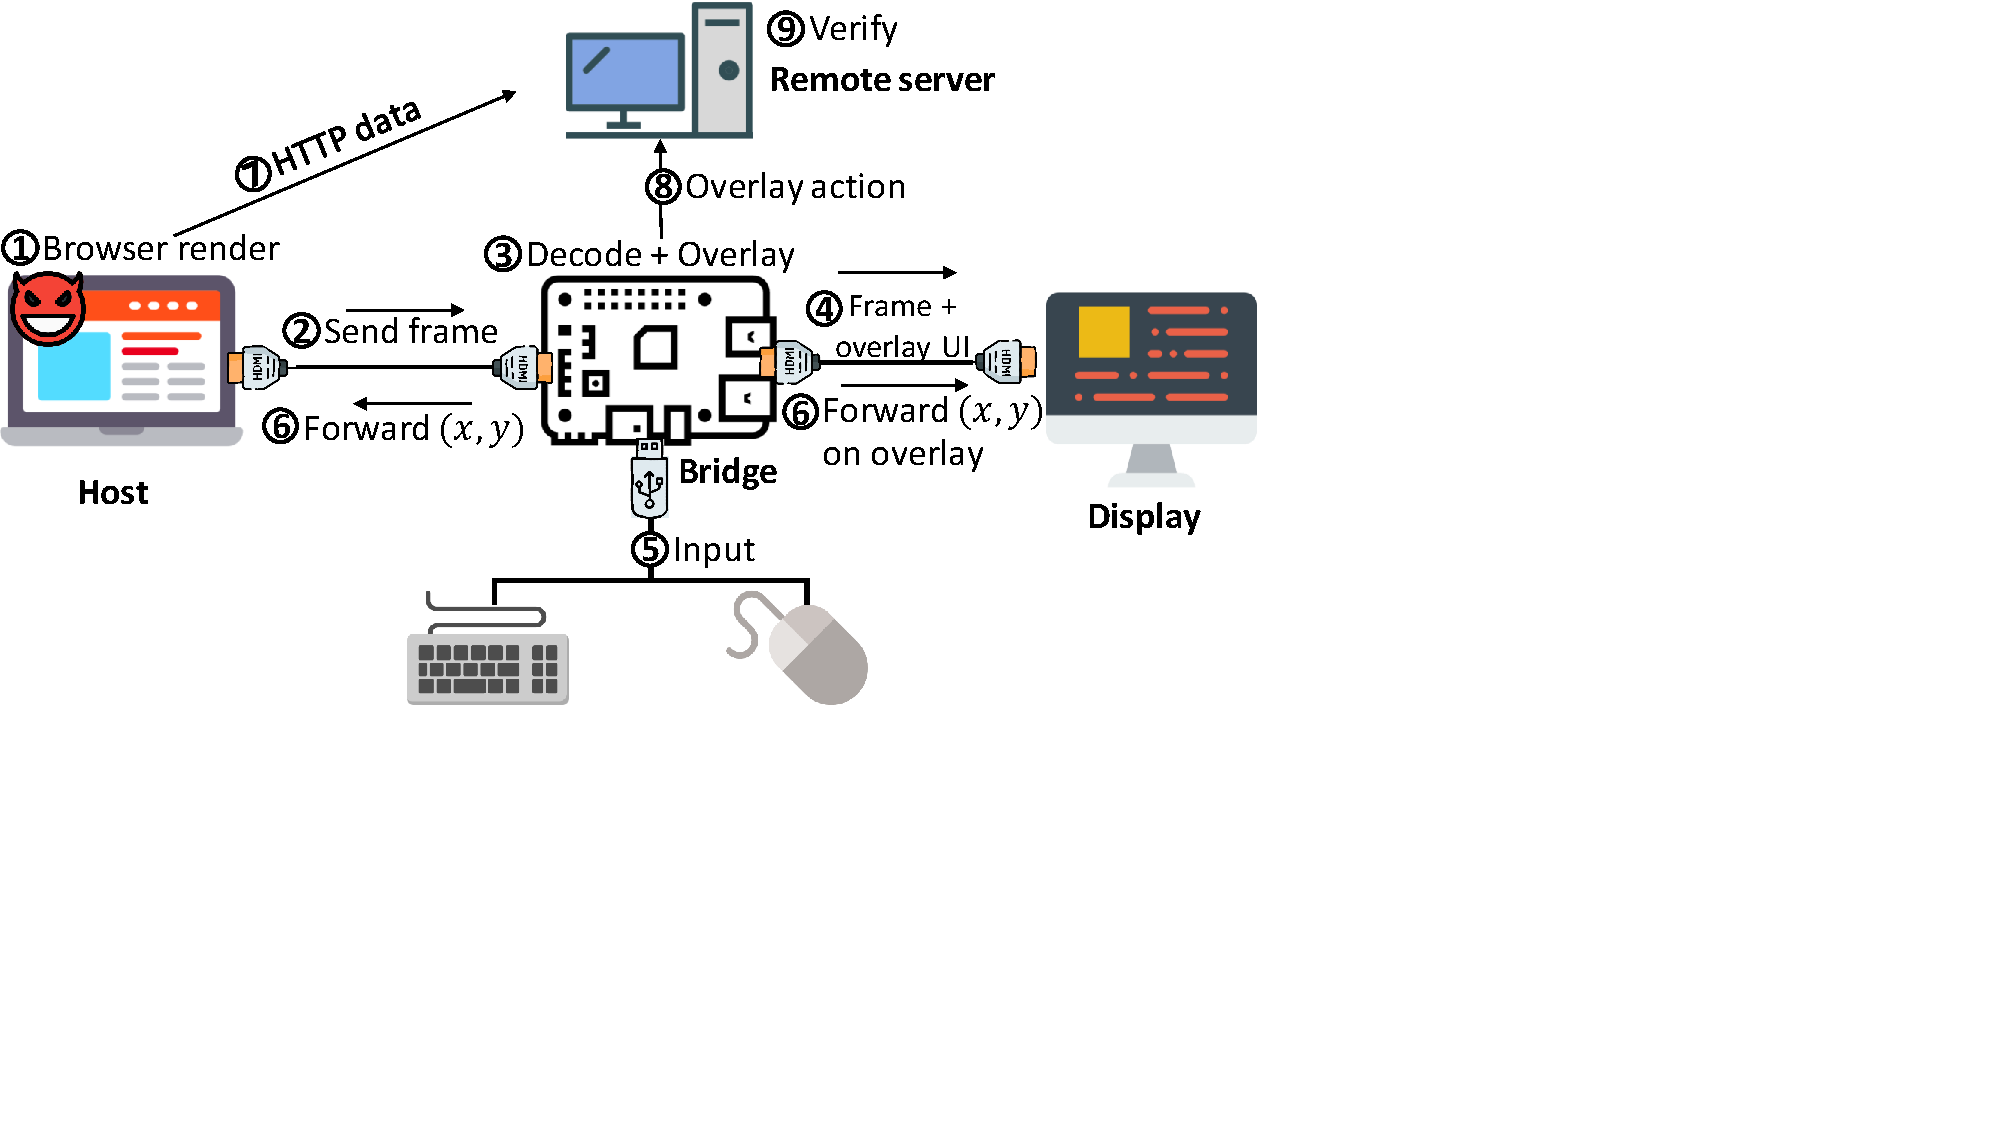
\includegraphics[trim={0 6.5cm 12cm 0}, clip, width=\linewidth]{systemDesign.pdf}
\caption{\textbf{High level flow of \name}}
\label{fig:systemDesign}
\centering
\end{figure}

\subsection{Main Protocol}
\label{sec:systemDesign:mainProtocol}

In the previous Sections, we explain the basic components of \name. Now in this Section, we describe the flow of \name protocol. The outline of \name is illustrated in Figure~\ref{fig:systemDesign}. In the flow, we assume that the user already clicked on a web link or write on the browser link field which web application to open. The steps are the following:


\begin{mylist}
  \item[\one] The browser on the host system receives the response from the remote server. The browser renders the webpage. Note, that the webpage contains the protected UI fields that are transformed by the \name JavaScript snippet to a QR code (detailed description in Section~\ref{sec:systemDesign:transformation}). The QR code contains a UI specification that can be decoded by the \device.
  \item[\two] The graphics driver sends the rendered frame to the \device over the HDMI channel.
  \item[\three] The \device intercepts the HDMI signal and decode the QR code to retrieve the UI specification. After the decoding of the QR code, the \device renders the bitmap corresponding to the specification.
  \item[\four] The \device send the HDMI frame with the UI overlay to the display device.
  \item[\five] After observing the HDMI frame and the overlaid UI, the user passes her input to the \device via the keyboard/mouse that is connected to the \device over the \usb interface.
  \item[\six] In this step, the \device forwards mouse traces (i.e., the $(\Delta x,\Delta y)$-mouse movements along $x$ and $y$ axis) to the host system. This is achieved as the \device enumerate itself as a composite HID (that includes both keyboard and mouse) to the host. Moreover, the \device also draw an overlay of the mouse pointer on its overlaid UI as the \device draws over the HDMI frames that are generated by the host. This provides a seamless user experience (Proof-of-pointer in Section~\ref{sec:systemDesign:analysis}).
  \item[\seven] When the user input her data to the host, the \device records her input data (Record phase in Section~\ref{sec:systemDesign:commit}).
  \item[\eight] The \name JavaScript snippet also acts as a upstream channel from the \device to the remote server (refer to Section~\ref{sec:systemDesign:communicationChannel}). Via this channel, the \device sends the signed user action to the remote server. This signed user action can be seen as the second factor for the integrity of the user input data. (Commit phase in Section~\ref{sec:systemDesign:commit})
  \item [\nine] The server verifies the data from the two channels that are submitted by the host and the \device. (Section~\ref{sec:systemDesign:serverSide})
\end{mylist}



\begin{figure}[t]
\centering
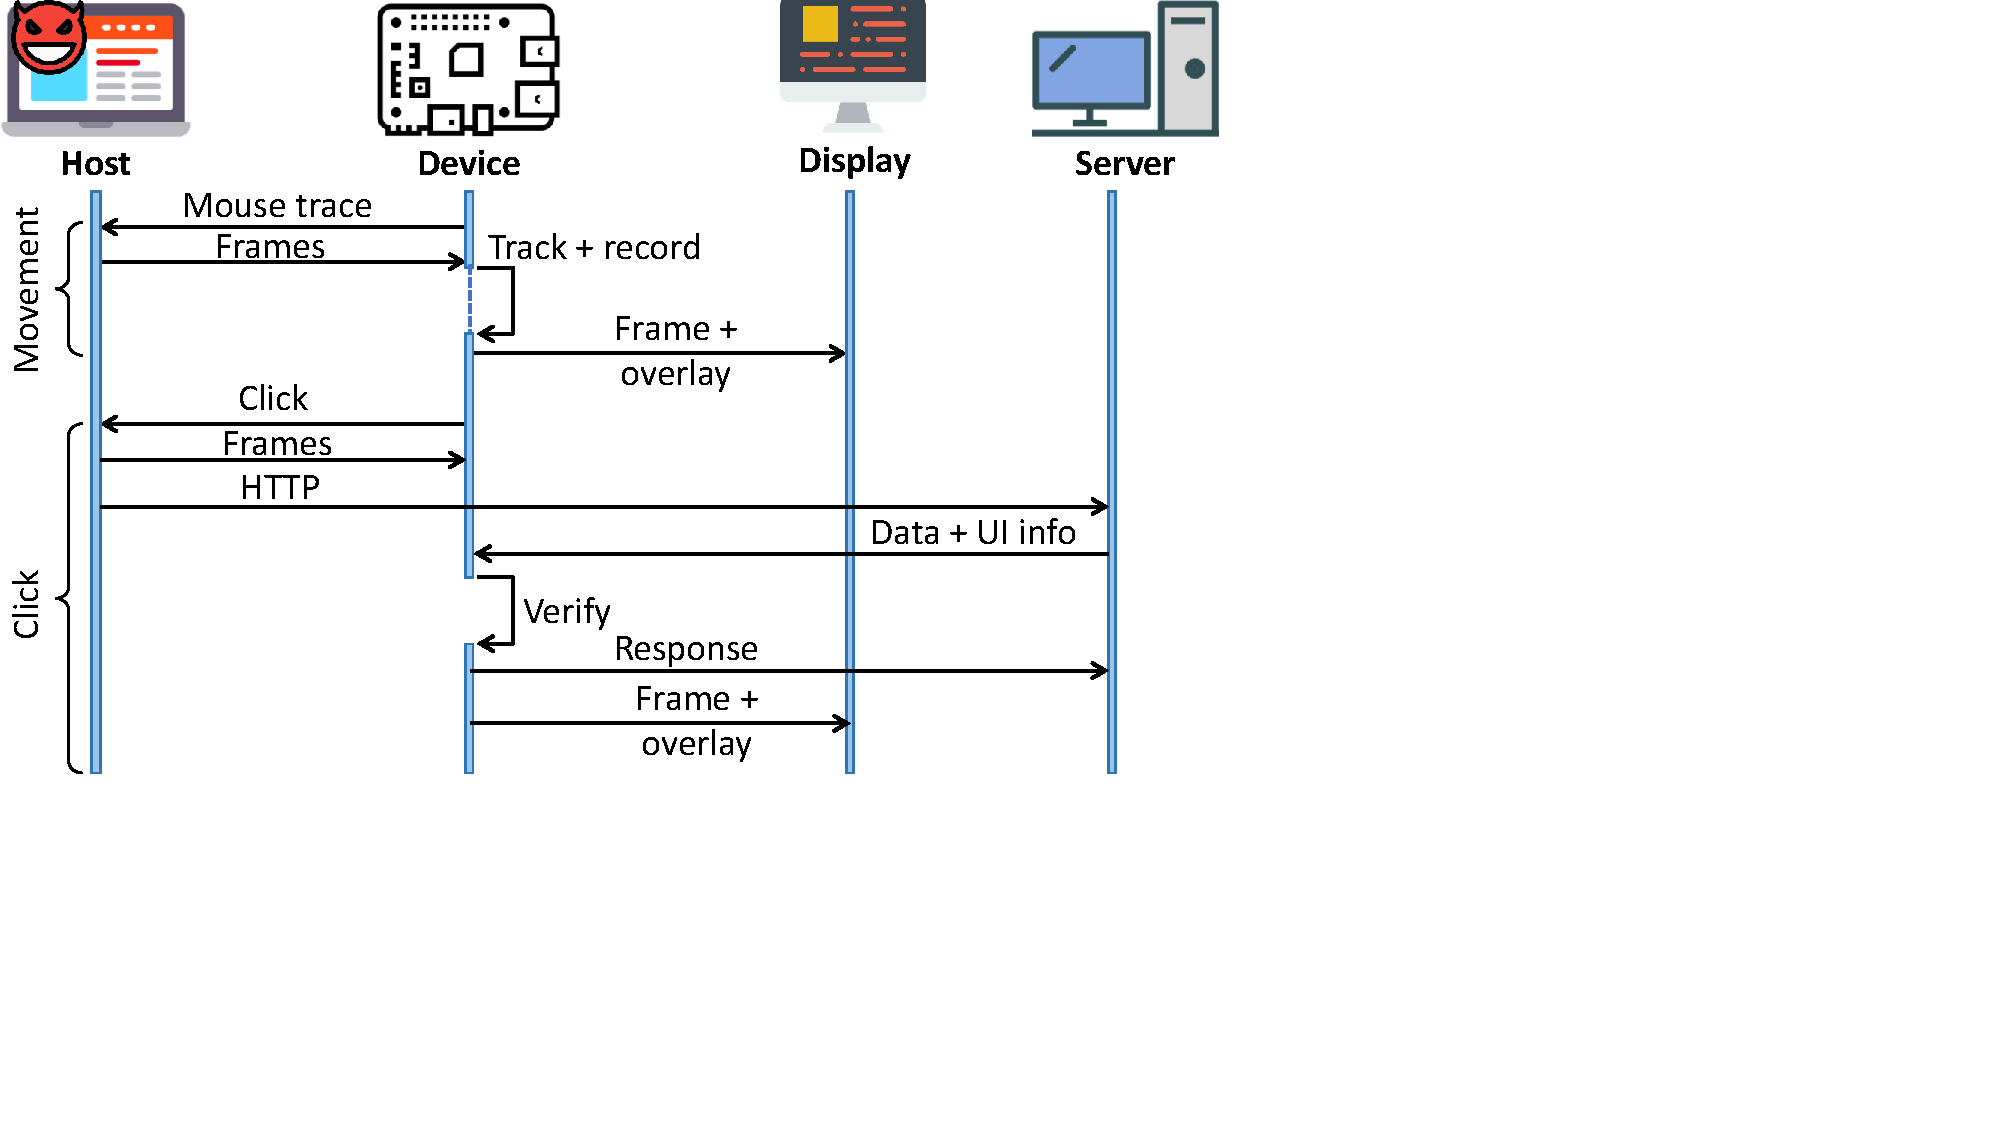
\includegraphics[trim={0 5.8cm 13cm 0}, clip, width=\linewidth]{flow.pdf}
\caption{Protocol}
\label{fig:protocol}
\end{figure}




\iffalse
\begin{figure}[t]
\centering
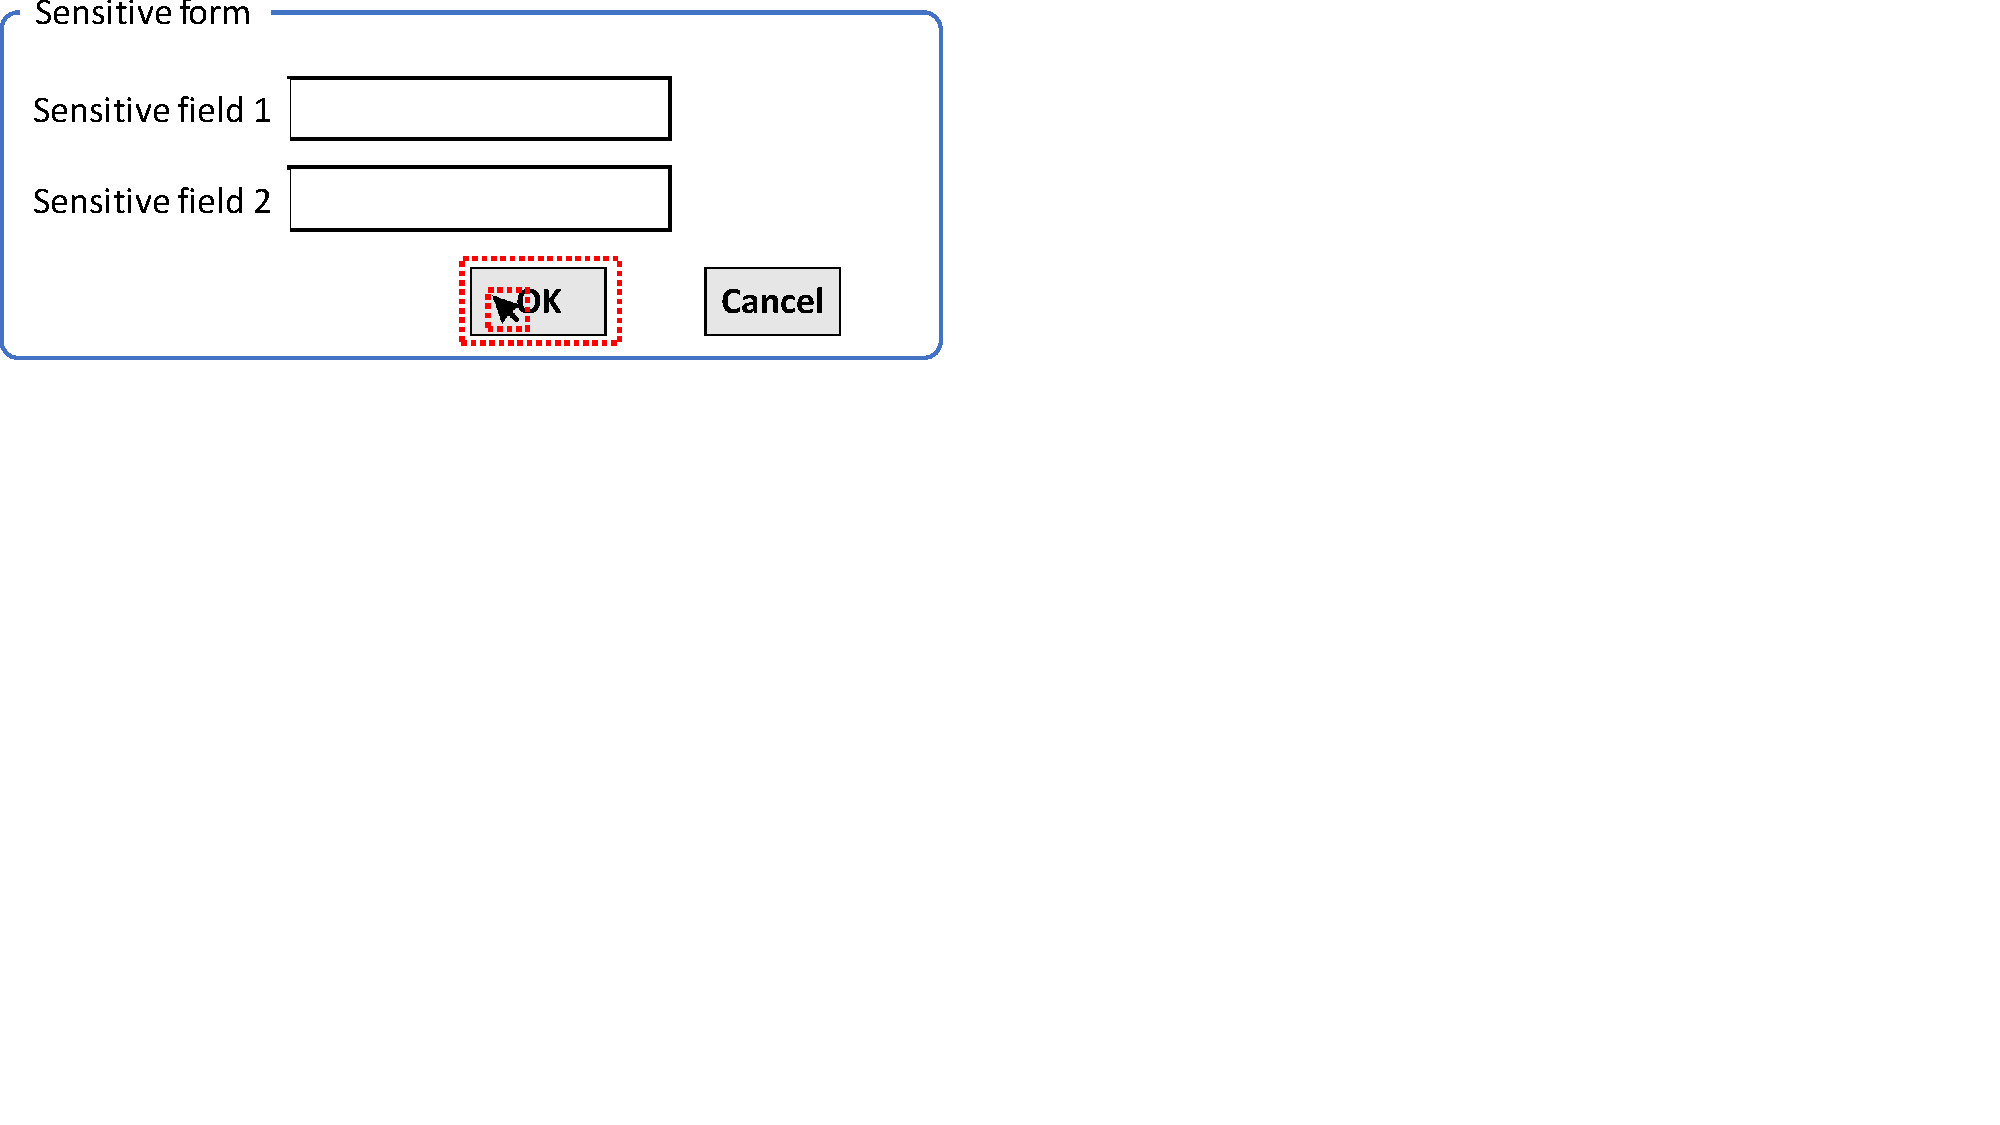
\includegraphics[trim={0 12cm 17cm 0}, clip, width=0.8\linewidth]{uiDetect.pdf}
\caption{Detection of the UI elements upon mouse click event in the incoming frame.}
\label{fig:uiDetect}
\centering
\end{figure}
\fi
% \begin{figure}
% \centering
% 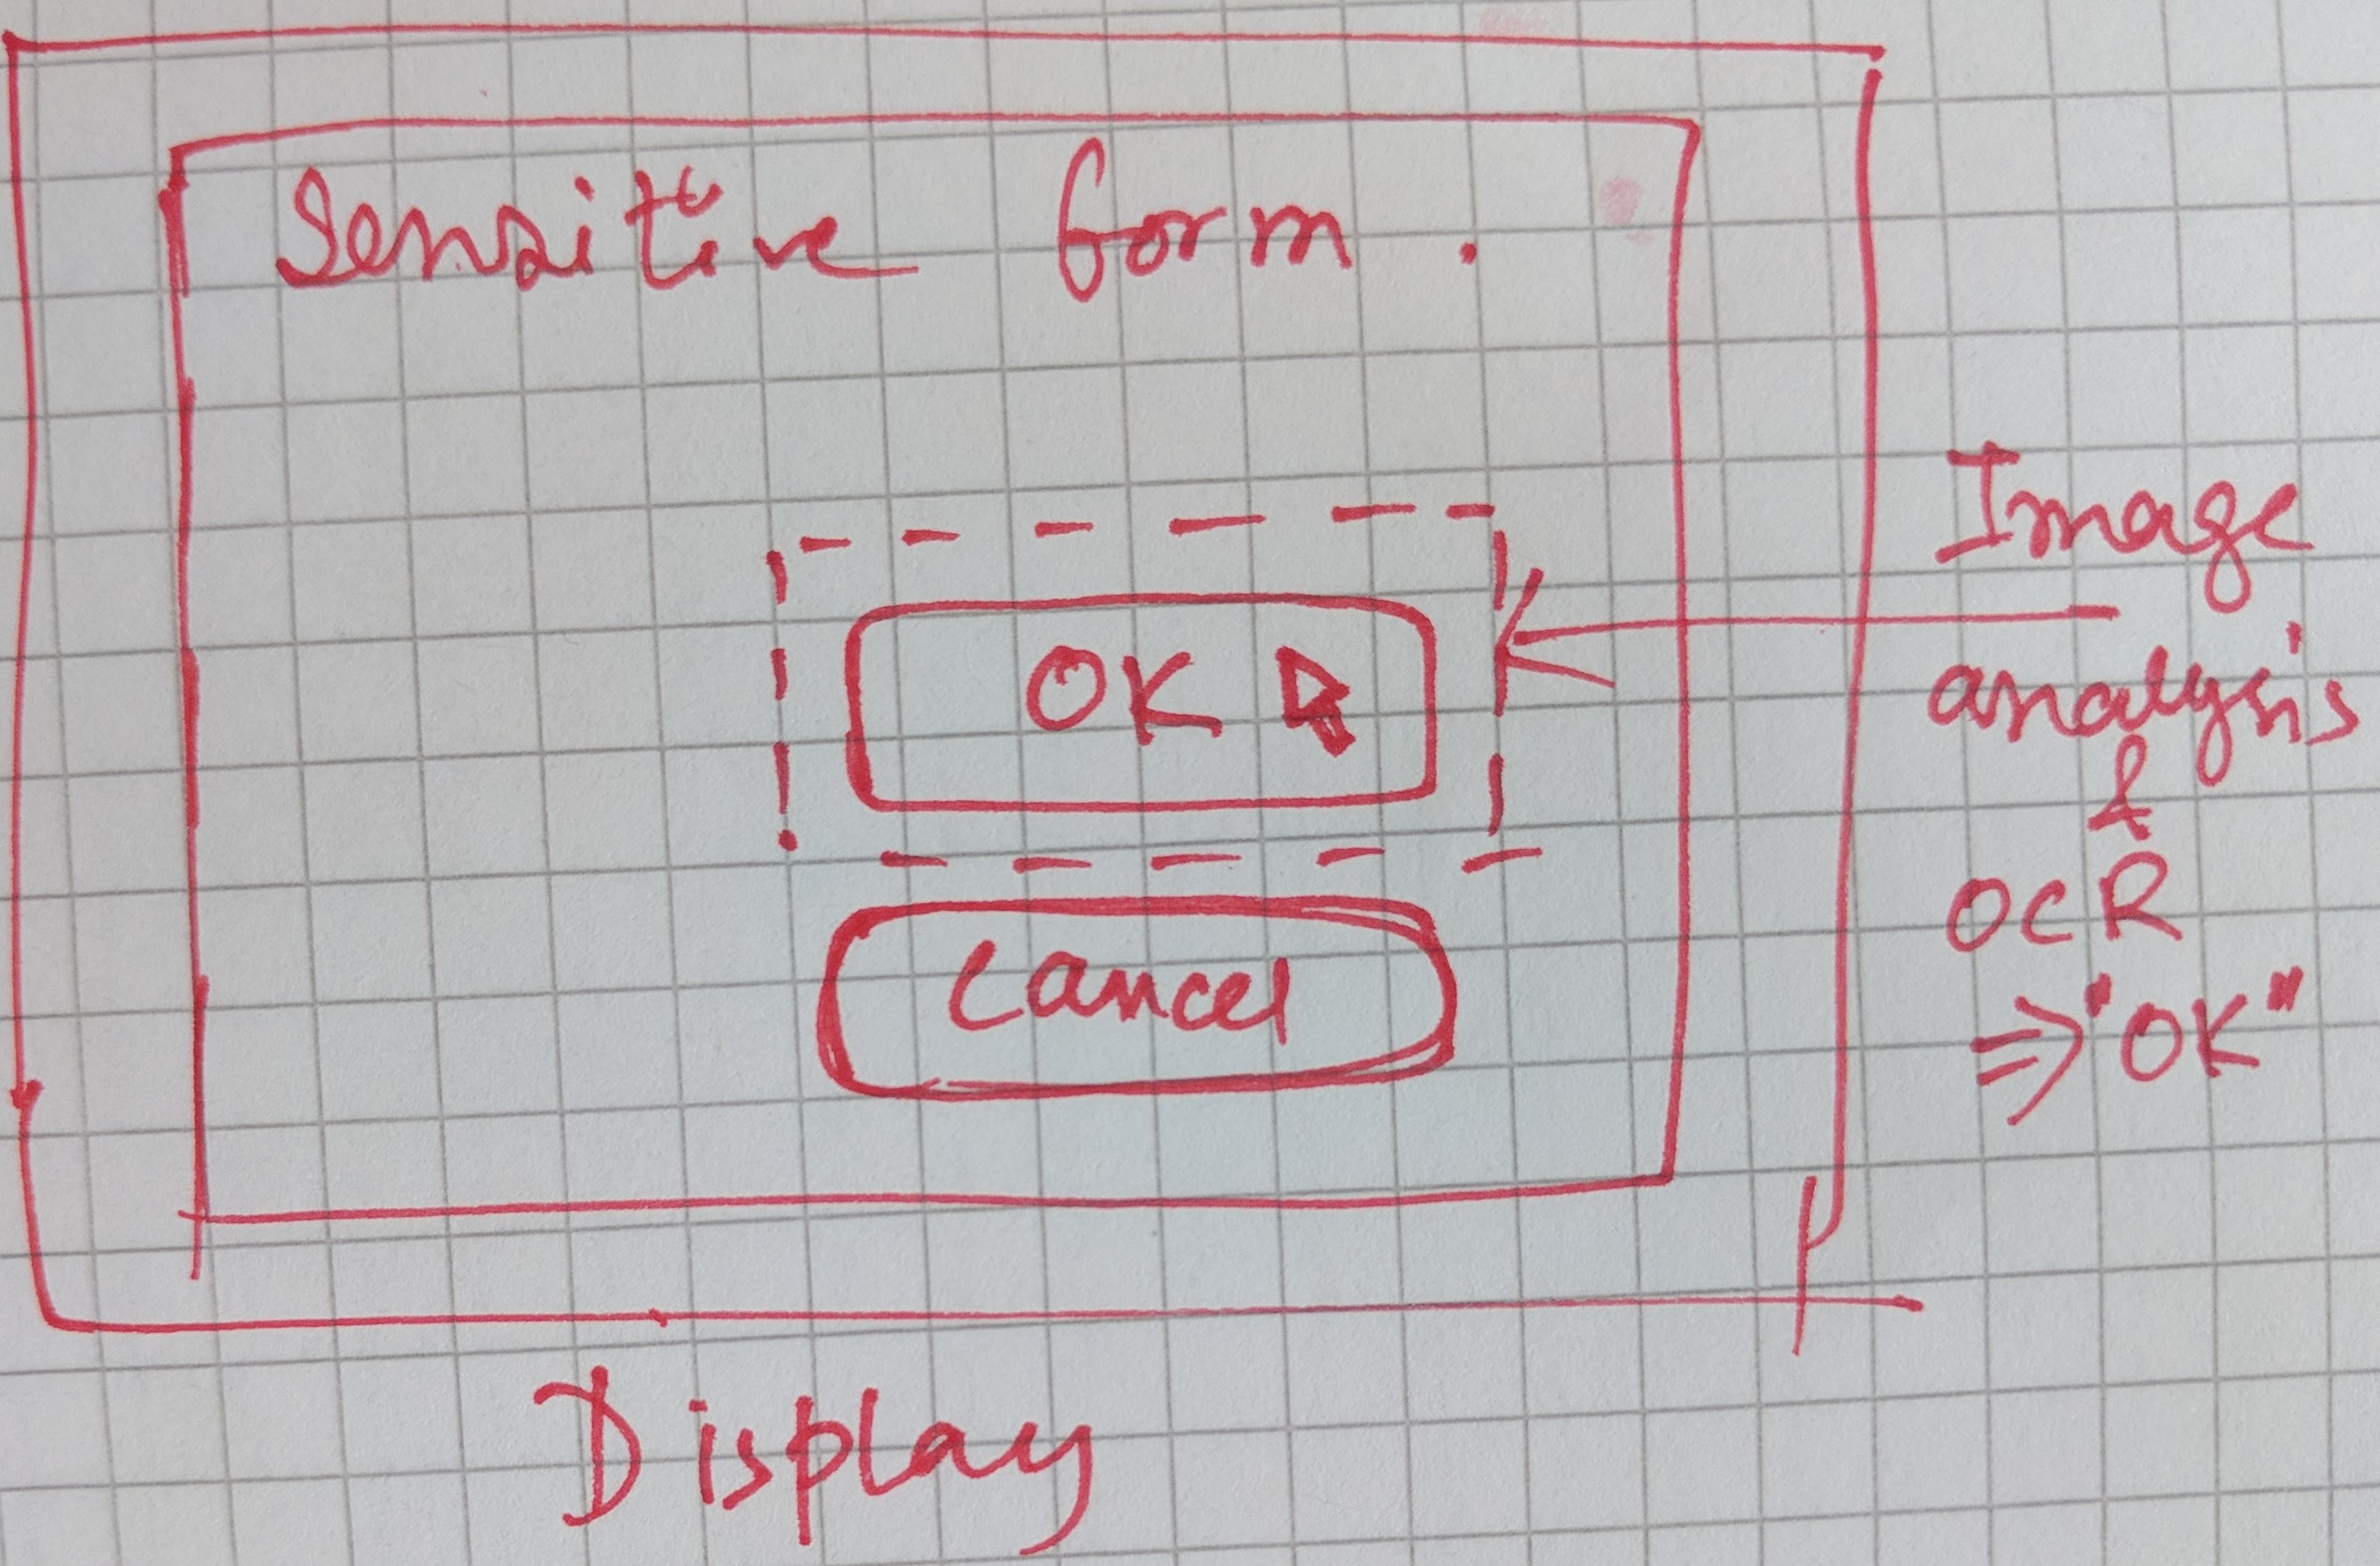
\includegraphics[width=\linewidth]{ui_detect.jpg}
% \caption{Detection of UI elements}
% \label{fig:uiDetect}
% \centering
% \end{figure}



\iffalse
\subsection{Detecting UI elements}
\label{sec:systemDesign:uiElements}

Detecting the UI elements triggers when the user clicks. The \device uses a square of $X$ square pixels around the mouse pointer and analyze the image. Figure~\ref{fig:uiDetect} illustrates an example of detecting the UI element from the captured frame. For example, if the user clicks on a button, the \device executes the image analysis on the part of the image to try to figure out if there is a button and parse the text. Additionally, the \device also sends the button text to the server. The server checks the data sent by the \device and the data received from the browser and compares them. In case there is a mismatch, the server notifies the \device and the \device overlays an error message on the screen. 
\fi

\begin{figure}[h]
\centering
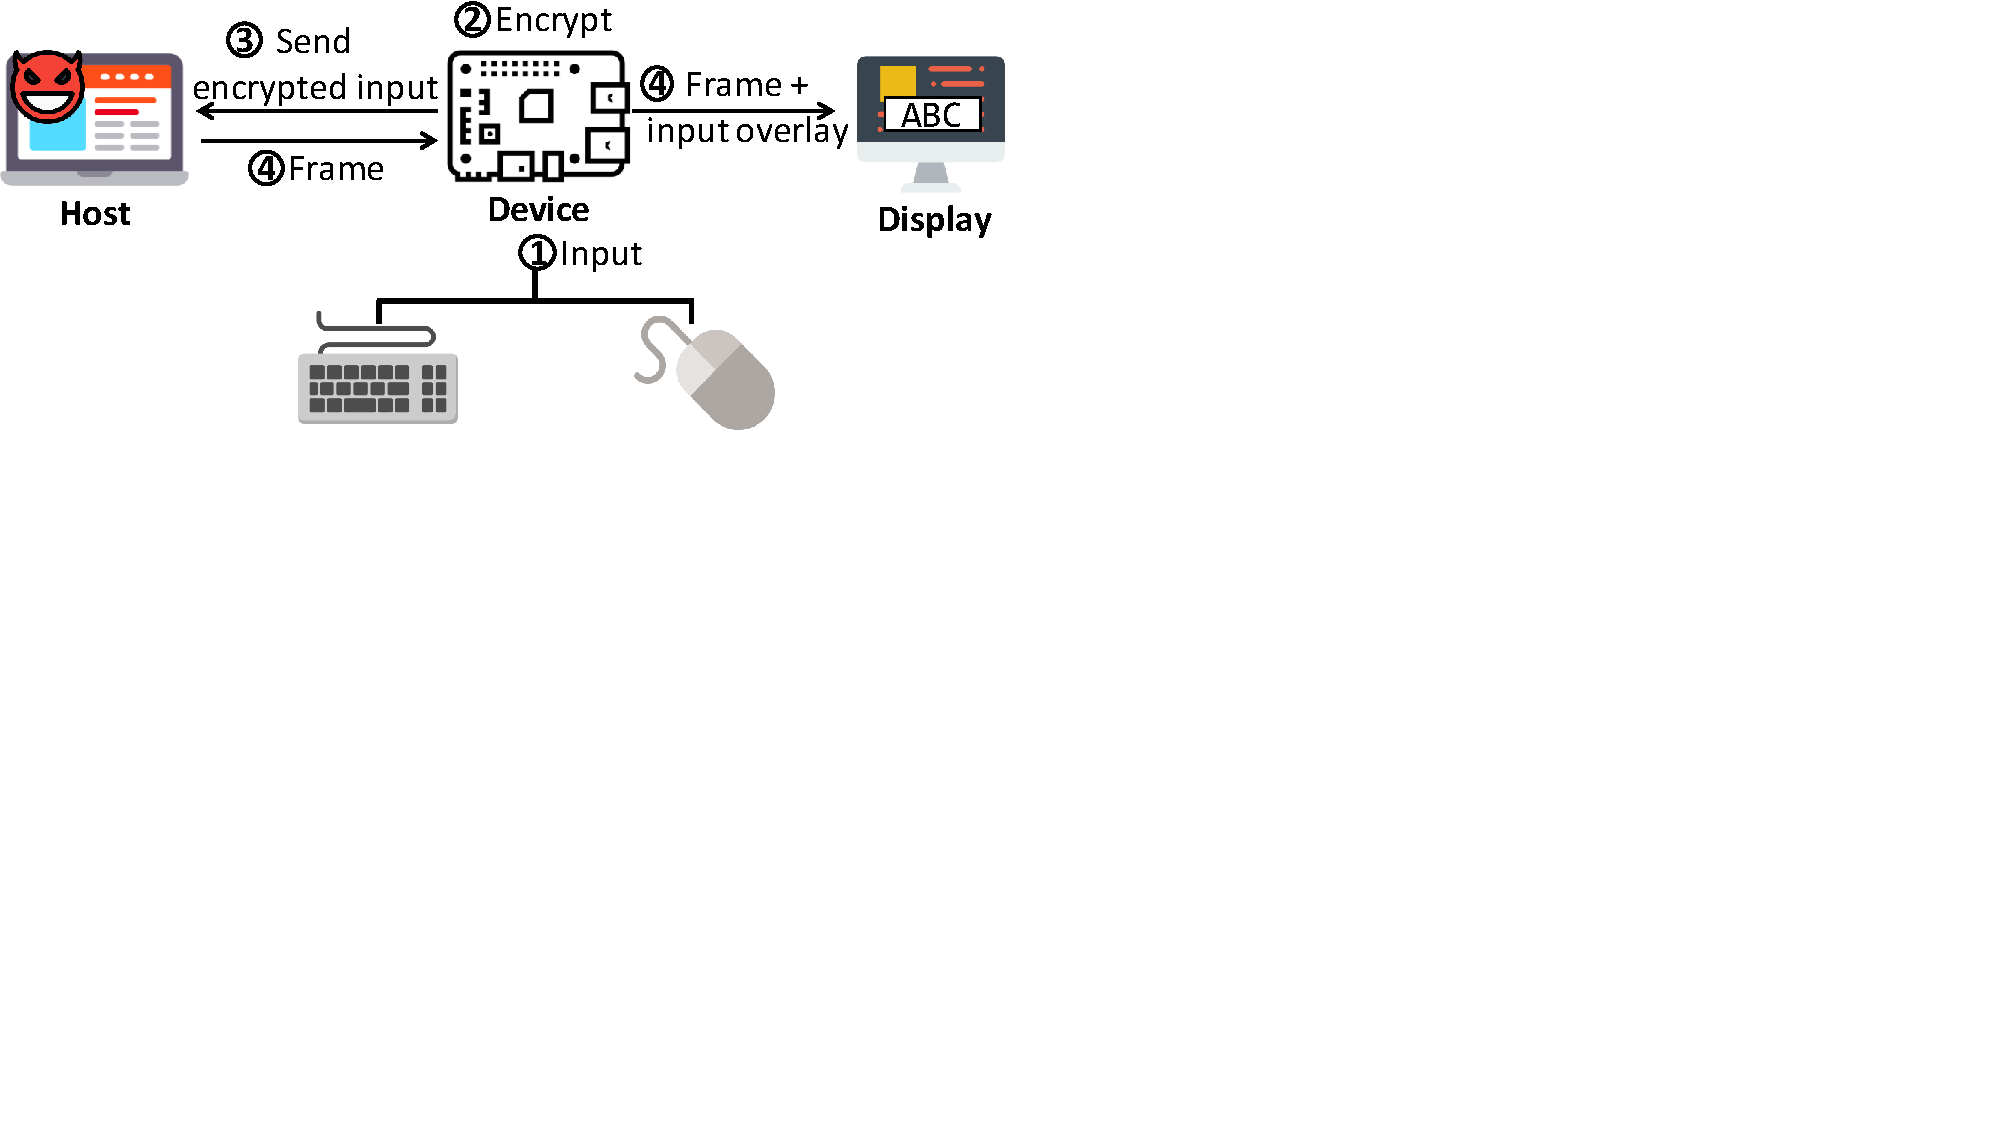
\includegraphics[trim={0 11cm 16.5cm 0}, clip, width=\linewidth]{inputPrivacy.pdf}
\caption{Input privacy}
\label{fig:inputPrivacy}
\centering
\end{figure}

